\section{SMACCMPilot: a High-Assurance Autopilot}
\label{sec:smaccmpilot}

\begin{figure}[ht!]
  \begin{center}
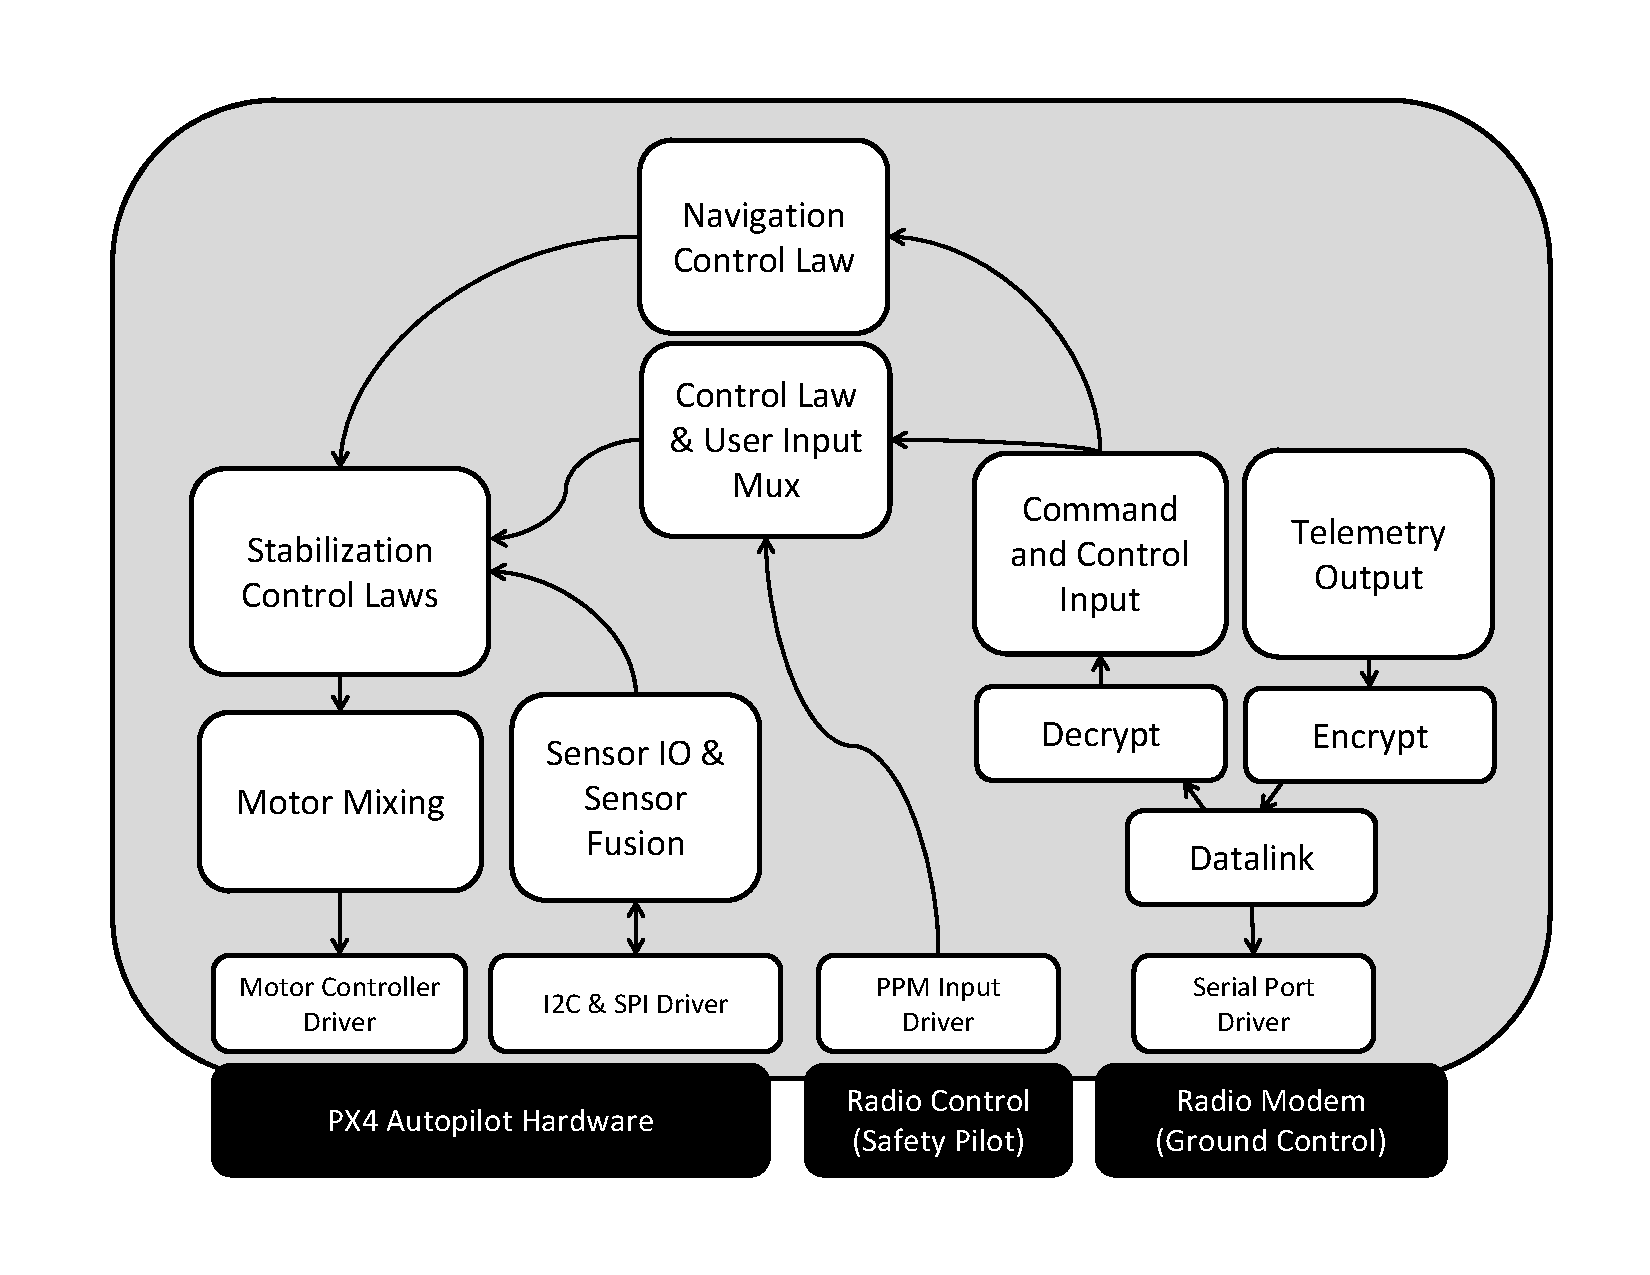
\includegraphics[width=8cm]{figures/smaccmpilot-diagram-jan14}
  \end{center}
\caption[SMACCMPilot software architecture]{
Simplified diagram of SMACCMPilot
software architecture. Tasks written in Ivory are shown as white boxes,
tasks implemented in legacy C++ code are gray boxes,
channels are arrows,
hardware components are black boxes.}
\label{fig:smaccmpilotSwArch}
\end{figure}

SMACCMPilot is an open-source (BSD Licensed) autopilot system for quadcopter
unmanned air vehicles (UAVs).
It is complete embedded system implemented with
the Ivory/Tower tools.
It includes low-level IO peripheral drivers, an encrypted
communication protocol stack, and several layers of control systems.

SMACCMPilot runs on open source flight controller hardware from the PX4
Autopilot project~\cite{px4-proj}. The hardware platform is
a custom printed circuit board with an ARM Cortex M4 microcontroller and the
sensors used to determine the orientation and altitude of the vehicle.


A simplified software architecture of SMACCMPilot is shown in
Figure~\ref{fig:smaccmpilotSwArch}.
The flight control software is primarily responsible for reading the sensors,
estimating the vehicle's attitude and position using sensor fusion, calculating
control outputs, and sending motor power commands to the motor controllers.
Higher level control loops manage navigation, and an encrypted command, control,
and telemetry link interprets ground station instructions, sends system state to
the operator, and permits online tuning of control loop parameters.

The result is a reasonably complex piece of embedded software. SMACCMPilot has
30 tasks connected by 47 channels, and 57 globally shared state variables. Most
of those shared state variables are control loop tuning parameters, which can be
modified by commands sent over the telemetry link.

SMACCMPilot was developed alongside the Ivory/Tower tools.  The complete system
took approximately 22 engineer-months to develop.  The low level drivers for the
system were written first in C, then transliterated to Ivory as the language
became mature enough to support them. We built a stack for command, control, and
telemetry, encapsulated in an encrypted packet protocol. A few components from
the ArduPilot open source project, the biggest of which is a 10kloc C++ library
for intertial sensor fusion, are still used inside SMACCMPilot.

\paragraph{Complexity comparison}
The SMACCMPilot application code is 10kloc of Ivory, the board support code
is 3kloc of Ivory, and the telemetry link binary packing and unpacking
code is a machine generated 10kloc of Ivory code. When compiled, the complete
application
is 48kloc of generated C~code, and depends on some external C libraries to
implement the operating system (4kloc) and other functions, such as sensor
fusion  This compares favorably to existing open
source flight controller systems.

As an example, we've selected two other systems which have a similar feature set
and run on similar hardware to SMACCMPilot - the ArduPilot
project\cite{apm-proj} and the PX4 project. Though, in
both cases, these systems have more high level functionality than SMACCMPilot,
they both implement all of the low level features to support similar (or
identical) microcontroller based flight controller boards, comparable low level
control laws, and implement the same MAVLink telemetry protocol.

The ArduPilot project is 60kloc of C++, uses three pseudo-threads (emulated by
interrupts on processors unsuitable for operating systems), and supports at
least four distinct autopilot hardware platforms. The PX4 Autopilot software
stack has 25kloc of C/C++ application code, 25kloc of C/C++ platform support
code, and depends on the large (50kloc+) NuttX operating system.

